\documentclass[man]{apa2}
\usepackage{pslatex}
\usepackage{amssymb}
\usepackage{graphicx}
\usepackage{color}
\usepackage{covington}
\usepackage[usenames,dvipsnames]{xcolor}
\usepackage{booktabs}
\usepackage{setspace}
% \usepackage{textgreek}
\usepackage{geometry}
\usepackage{pdflscape}
\usepackage{array}
\usepackage{floatrow}
\usepackage{fancyhdr}
\usepackage{apacite}
\bibliographystyle{apacite}
\geometry{reset, letterpaper, height=9in, width=6in, hmarginratio=1:1, vmarginratio=1:1, marginparsep=0pt, marginparwidth=0pt, headheight=15pt}

\fancyhf{} % sets both header and footer to nothing
\renewcommand{\headrulewidth}{0pt}

\newcolumntype{C}[1]{>{\centering\let\newline\\\arraybackslash\hspace{0pt}}m{#1}}

\title{The trouble with quantifiers: Exploring children's deficits in scalar implicature}

\threeauthors{Alexandra C. Horowitz*}{Rose M. Schneider*}{Michael C. Frank}
\threeaffiliations{Department of Psychology, Stanford University}{Department of Psychology, University of Pennsylvania}{Department of Psychology, Stanford University}

\shorttitle{The trouble with quantifiers}
\rightheader{The trouble with quantifiers}


\acknowledgements{The two first authors contributed equally to this paper. We gratefully acknowledge Tamara Mekler for her assistance in data collection, the staff and families at Bing Nursery School, as well as David Barner for guidance on the Give-Quantifier task.

~\\

\noindent Please address all correspondence to Rose M. Schneider, University of Pennsylvania, Department of Psychology, Levin Building, 425 S. University Avenue, Philadelphia, PA 19104. E-mail: \texttt{rosems@sas.upenn.edu}.}

%\begin{document}
%\maketitle

%\pagestyle{fancy}
%\rhead{The trouble with quantifiers \ \ \thepage}
\begin{document}
\maketitle
%~\\
%~\\
%~\\
%\shorttitle{The trouble with quantifiers}
%\rightheader{The trouble with quantifiers}
%\begin{center}
%\textbf{The trouble with quantifiers: Exploring children's deficits in scalar implicature}
%\end{center}
%\author{  }
%\affiliation{  }
\newpage
\begin{center}
\textbf{Abstract}
\vspace{5 mm}
\end{center}
\noindent
%abstract now in third person
Adults routinely use the context of utterances to infer a meaning beyond the literal semantics of their words (e.g., inferring from ``She ate some of the cookies'' that she ate some, but not all). Contrasting children's (N = 209) comprehension of scalar implicatures using quantifiers with contextually-derived ad-hoc implicatures revealed that four-- to five--year-olds reliably computed ad-hoc, but not scalar, implicatures (Experiment 1). Unexpectedly, performance with ``some'' and ``none'' was correlated (Experiments 1 and 2). An individual differences study revealed a correlation between quantifier knowledge and implicature success (Experiment 3); a control study ruled out other factors (Experiment 4). These findings suggest some failures with scalar implicatures may be rooted in a lack of semantic knowledge rather than general pragmatic or processing demands.

%first-person abstract
%We contrasted children's (N=209) comprehension of scalar implicatures with quantifiers and ad-hoc implicatures that relied only on contextual details. . Unexpectedly, performance with ``some'' and ``none'' was correlated (Experiment 2). An individual differences study revealed a correlation between quantifier knowledge and implicature success (Experiment 3); a control study ruled out other factors (Experiment 4). Our findings suggest some failures with scalar implicatures may be rooted in lack of semantic knowledge rather than general pragmatic or processing demands.

~\\

\noindent
Keywords: scalar implicature, pragmatics, development

%\shorttitle{The trouble with quantifiers}
%\rightheader{The trouble with quantifiers}
%\acknowledgements{
%
%~\\
%
%\noindent }

%\begin{document}
%\maketitle
\newpage

\section{Introduction}
Human language users have a remarkable ability: We can infer a speaker's intended meaning even when it is not explicitly conveyed by the literal meanings of the words in the utterance. For example, an adult who hears ``I ate \emph{some} of the cookies'' would expect that the speaker did not eat \emph{all} the cookies. Similarly, an adult who hears ``I ate the \emph{sugar} cookies,'' would most likely assume that the speaker ate \emph{only} the sugar cookies, and not the other varieties. In both cases, listeners are inferring a speaker's intended meaning not from what was said, but from what was \emph{unsaid}.

Such pragmatic inferences are a critical part of language use \cite<e.g.>{clark1996,levinson2000,frank2012}. Thus, to become fluent language users, children must not only learn the literal meanings of the words in an utterance, but also how to leverage these meanings to make inferences beyond the literal sense of the utterance. In the two statements above, a speaker employs a weaker literal description to implicate that a stronger alternative is false. The first statement requires the listener to make a \emph{scalar implicature}, which relies on lexical scales such as quantifiers (``some'' vs. ``all'') or modals (``possibly'' vs. ``definitely'') \cite{horn1972}. The second statement requires an \emph{ad-hoc implicature}, in which a stronger description is negated by a contextually weaker description. Here, we use ``ad-hoc implicature" (rather than ``generalized'' or ``particularized''; \citeNP{grice1975}) as a term of convenience to describe contextually-supported inferences. In both instances, the listeners must reason not only about the semantics of the literal utterance, but also of the alternatives implicated in its pragmatic reading.

Both scalar and ad-hoc implicatures are abundant in language; it would be time-consuming and computationally costly to both speakers and listeners if all intended meaning had to be conveyed literally. Because of this abundance, the ability to make pragmatic inferences is a critical component of linguistic competence, permitting rich knowledge about intended meaning while minimizing speaker effort \cite{grice1975,horn1984}. How does such a crucial linguistic skill develop, and what can it reveal more broadly about the developmental trajectory of the semantics--pragmatics interface \cite{papafragou2003}?

Although much research has been devoted to the topic, when and how children gain the ability to make scalar implicatures remain unclear. While adults sometimes incur a processing cost in computing scalar implicatures along quantifier lexical scales like  $<${\sc some, all}$>$ \cite{bott2004,grodner2010,huang2009b}, they reliably compute implicatures in a wide variety of situations. In contrast, early investigations showed that children's accuracy on these same scales was variable even until fairly late in development \cite{noveck2001}. This result was intriguing because implicatures are an important case study for children's general pragmatic reasoning. The finding that even elementary-aged children struggled with certain types of pragmatic judgments suggested a surprising disconnect between pragmatics and other aspects of language development. In recent investigations, however, children have shown a graded pattern of successes and failures across different tasks \cite<e.g., >{guasti2005,papafragou2003, papafragou2004, skordos2016}. Five-year-olds show evidence of recognizing that pragmatically-infelicitous statements deserve smaller rewards, when given a graded---rather than binary---judgment task \cite{katsos2011}. And some three- and four-year-olds can make ad-hoc (contextual) implicatures in a stripped--down referent-selection paradigm \cite{stiller2015}. So although some methods still show notable failures \cite<e.g.,>{huang2009}, the evidence is more mixed as to what children's abilities are and precisely what causes the observed deficits.

While much progress has been made in this area, one weakness of the current literature is its diversity (see Table \ref{tab:lit_review} for a non-exhaustive summary of influential experimental papers). First, a wide range of methods and measures---from referent selection to felicity judgment---have been used to assess children's implicature abilities. Second, most previous studies have targeted relatively wide age bins (12--18 months or wider), ranges that do not allow for precise developmental comparisons between studies. And finally, other paradigm-level differences might lead to varying levels of performance. For example, recent work indicates that the use of the partitive (e.g., ``\emph{Some} of the cookies'') is a particularly strong cue for adults' scalar implicatures \cite{degen2015b}, but studies vary in their use of this construction.

Thus, one goal of our current work is to consolidate insights from the previous literature by providing a direct comparison between ad-hoc and scalar implicatures in a simple referent selection task. This comparison allows for strong inferences about developmental differences between scalar and ad-hoc implicatures computation. Additionally, a second goal of our current work is to explore theoretical hypotheses about the source of children's surprising scalar implicature failures. We follow previous work in suggesting that, if children succeed in ad-hoc implicatures and fail in scalar implicatures, it is very unlikely that a general pragmatic deficit explains previous findings. The next section explores another possible class of explanations.

\subsection{Explaining Children's Failures in Scalar Implicature}

The \emph{Alternatives Hypothesis} suggests that children's performance may have less to do with general pragmatic knowledge per se, and more to do with their knowledge of the particular scales on which implicatures are computed. Barner and colleagues \cite{barner2010,barner2011} suggested that children's ability to compute scalar implicatures relies on their recognition of the relevant lexical alternatives (e.g., that use of the weaker term ``some'' conveys a direct contrast with the stronger alternative ``all,'' thus implying \emph{some but not all}).  In other words, children's pragmatic inferences rely on their ability to consider alternatives to the words chosen by the speaker. Hence, even in supportive paradigms, if children cannot bring to mind ``all'' when reasoning about ``some,'' they will fail to make an implicature.

%NOTE - ADD MORE DISCUSSION ABOUT ALTERNATIVES HYPOTHESIS - EMPIRICAL TESTS
Previous research has provided a number of tests of this hypothesis. First, children's performance in implicature tasks increases when they have stronger access to specifically lexical alternatives. \citeA{skordos2016} found that making scalar alternatives salient with a blocked design  (e.g. ``all'' trials presented before ``some'' trials) increased scalar implicature computation in English-speaking 5-year-olds. Second, even when lexical alternatives are not presented directly, the use of more supportive paradigms or designs could be helpful. In particular, if referents corresponding to particular lexical alternatives are present on each trial, the presence of these referents could facilitate reasoning about alternatives. Supporting this idea, preschoolers (3;6--5;0) showed some preliminary evidence of computing scalar implicatures for quantifiers in a forced-choice paradigm where different quantificational scenarios were pictured \cite{miller2005}. And 4--5-year-old children could reason about ad-hoc scales both in a forced-choice paradigm \cite{stiller2015} and in a truth-value paradigm \cite{barner2011} when the relevant alternative objects were present in the trial context. Finally, recent work on inferences about disjunction argues that children's struggles are due to failures in generating an adult-like set of alternatives, rather than general semantic or pragmatic deficits \cite{singh2016,tieu2016}.

%NOTE - HERE WE SHOULD TALK MORE ABOUT QUANTIFIERS, WHY THEY ARE DIFFICULT
On the other hand, this body of research leaves open another possible explanation. Perhaps the problem is not with inferential alternatives generally, but instead a specific issue with quantificational alternatives. Perhaps children have trouble summoning to mind quantificational alternatives because---at varying times in development---they either 1) do not know the quantifiers, 2) do know them but cannot process them effectively, or 3) know them and can process them but have not grouped them into sets of lexical alternatives. In some sense, all three of these possibilities are consistent with the spirit of the Alternatives Hypothesis, but problems 1 and 2 are perhaps more specific to quantifier meaning than otherwise supposed. Such quantifier-specific accounts might be most relevant for younger children. We return below to the idea that these accounts might not be mutually exclusive but might instead apply differently at different ages.

Supporting this line of reasoning, quantifiers are a difficult lexical class for children to acquire. Unlike many other lexical classes (e.g., colors), quantifiers are not mutually exclusive with one another (and hence, they produce implicatures). In addition, quantifier semantics are relative to the total set size. For example, in a set size of 8, the quantifier ``some'' can be used felicitously to describe anywhere from 2 -- 7 objects \cite{barner2009} (and truth-functionally to describe sets 1 -- 8), although adult responses tend to center around the set-size mean \cite{franke2014}. These difficulties are seen in an experiment by \citeA{hurewitz2006},  where 3--4-year-olds were only 75\% correct in choosing the referent of ``all'' in a four-alternative forced choice. Thus, perhaps the problem lies specifically in the semantics of quantificational alternatives, rather than alternatives in general.

\subsection{The Current Study}

In four experiments, we explored these ideas about the determinants of performance in implicature tasks using a novel paradigm. We designed a simple referent selection task in which children were asked to select which of three book covers they thought the experimenter was describing. This task gave children access to the visual alternatives in each trial (the three book covers) and the lexical alternatives across trials (either ad-hoc or scalar descriptions). Our design allowed us to counterbalance trial types (ad-hoc vs. scalar descriptions, crossed with implicature vs. unambiguous control targets) fully across participants, to examine both within-subject patterns of responses and between-subject developmental patterns, while also reducing task demands.

In Experiment 1, we included both ad-hoc and scalar descriptions with implicature and control trials for each. Four--year-olds were at ceiling on ad-hoc trials \cite<similar to previous work, e.g.>{stiller2015}, but their performance on scalar implicature trials was very low. In Experiment 2, we omitted ad-hoc trials, and found developmental increases in performance for all quantifiers, with higher performance on implicature trials for 4-year-olds in this scalar-only version. In both Experiments 1 and 2, we also found an unexpected result: Children's pattern of responses on scalar implicature trials was bimodal and strongly correlated with their performance on ``none'' trials. This correlation suggested a general source of difficulty in comprehending these quantifiers beyond simply failing to make a scalar implicature.

We further explored this correlation in Experiment 3 with an individual differences study. We measured quantifier knowledge with a separate paradigm \cite{barner2009}, and additionally assessed the alternative hypothesis that inhibitory control development, rather than quantifier alternative knowledge, might underlie the correlation between ``none" and implicature performance; we found no evidence for this interpretation. In Experiment 4, we tested the hypothesis that the salience of the \emph{some--all} contrast might have been diminished by the inclusion of the strong alternative ``none'' in our implicature task.  Contra this hypothesis -- and consistent with previous work \cite{skordos2016} -- including ``none''  actually \emph{facilitated} scalar implicature computation.

Overall, our findings suggest that while preschoolers' computation of scalar implicatures can be supported by stronger recognition of the lexical alternatives, some of their earlier failures are likely rooted in difficulty understanding the relevant quantifiers.

\section{Experiment 1: Ad-hoc and scalar implicature computation in children}

Our novel task used was designed to investigate both ad-hoc and scalar items with one set of visual stimuli presented in the same order to all participants; however, the particular target words for each trial (ad-hoc or scalar) were counterbalanced across participants. Thus, we could directly compare children's performance on both ad-hoc and scalar implicatures in a single experimental session. In Experiment 1, we included both ad-hoc and scalar implicatures. In all scalar items, we used a partitive construction (e.g., ``\emph{Some} of the pictures are cats'') to increase the likelihood of making an implicature \cite{degen2015}. All stimuli, data, and analyses for this and subsequent experiments are available in a version-controlled, public repository at \url{https://osf.io/mucf9}.

\subsection{Methods}

\subsubsection{Participants}

Table \ref{tab:exp_1_demo} shows the demographic information for a planned sample of 48 children recruited from a university preschool. The preschool is an English language school serving a high socioeconomic status and high educational achievement population. Children included in the sample were native speakers of English. Ethnicity information was not recorded for this sample. Two children were excluded from the final sample for not completing the task, and one additional child was excluded due to experimenter error. No child completed more than one session of the task. One participant has one trial excluded due to experimenter error.

%These children were drawn from two age groups: 24 4.0 -- 4.5-year-olds (M = 4;2, median = 4.19, SD = 0.14) and 24 4.5 -- 5.0-year-olds (M = 4.74, median = 4.73, SD = .16).

\subsubsection{Stimuli}

Experimental stimuli consisted of 18 sets of three printed pictures of book covers, each featuring four familiar items. In each trial, one book cover contained four items of the same kind (e.g., four cats), another book cover contained four items of another kind (e.g., dogs), and the final cover contained two items of a new set and two items repeated from one of the other book covers (e.g., two birds and two cats). An example of the stimuli can be seen in Figure \ref{fig:demo}.

\subsubsection{Procedure}

Participants were tested in individual sessions in a quiet room at their nursery school. The experimenter introduced the study as a guessing game, and explained that the child would receive a hint about a single book cover. The experimenter emphasized that the child would only receive one clue, and she must use that clue to make her decision. All participants saw image sets (three books) in the same order; however, target location was counterbalanced across conditions. Description condition and trial-type were further randomized across participants, and were spaced to avoid immediate repeat trial types. Table \ref{tab:scripts} shows the breakdown of trial types and sample scripts. Children received only neutral feedback after the training trial.

Prior to test trials, children saw a practice trial with three book covers, each displaying a single unique and familiar item. At the start of the practice trial, the experimenter said ``On the cover of my book, there's a TV.'' After children successfully completed the practice, they proceeded to 18 test trials. At the beginning of every trial, the experimenter provided the child with either an ad-hoc or scalar description, and instructed the child to point to the book she was describing. If the child pointed to more than one book, or the response was otherwise ambiguous, the experimenter emphasized again that she was talking about just one book, and that the child should choose the single book she was describing.

In ad-hoc trials (eight total), the experimenter's descriptions of the target book used the names of the pictured objects, providing contextual support for the target. Ad-hoc control trials referred to an unambiguous target (e.g., ``On the cover of my book, there are dogs'' in Figure \ref{fig:demo}), while implicature trials required the child to reason about the speaker's meaning given an ambiguous utterance (e.g., ``On the cover of my book, there are cats,'' which could refer to either the book containing only cats or the book containing cats and birds). In these critical trials, children had to understand that the speaker could potentially be talking about either the book with four or two of the named object, but that by opting to describe only one kind of object she was referring to the cover with four of the same object; otherwise, she would have mentioned both kinds of objects, or the ones unique to that cover (i.e., birds).

In scalar trials (ten total), the experimenter described the target book with quantifiers. For scalar items, control trials referred to unambiguous targets with the quantifiers ``all'' and ``none'' (e.g., ``On the cover of my book, \textit{all/none} of the pictures are cats'') or an unambiguous referent of ``some'' (e.g., ``On the cover of my book, \textit{some} of the pictures are birds.''). On critical scalar implicature trials, the experimenter used the weak quantifier ``some'' to reference the item pictured across two book covers (e.g., ``On the cover of my book, \textit{some} of the pictures are cats.''). These trials required the child to reason that because the speaker used the weak quantifier ``some,'' she must be referring to the book picturing only two of the named target, or else she would have used the stronger quantifier ``all.''

\subsection{Results}

Children performed at ceiling on ad-hoc implicature trials, but struggled on both scalar implicature and ``none'' trials. Accuracy on all trial types is plotted in Figure \ref{fig:exp1_perf}. On implicature trials, children's responses were coded as correct if they selected the image consistent with the implicature: the single item (e.g., cats) on the ad-hoc trials, and the mixed item (e.g., cats and birds) on the scalar trials. On other trials, responses were coded as correct if the cover was consistent with the description (e.g., selecting the cover with four dogs in response to the description ``None of the pictures are cats.'').

Children's performance with ad-hoc implicatures was consistent with previous research suggesting that they can succeed making such implicatures when they have access to the lexical alternatives \cite{stiller2015}. This result provides evidence that our novel paradigm is an appropriate measure for such items -- despite employing a weak ad hoc utterance ``there are cats,'' which would be expected to produce less pragmatic effect than the stronger definite determiner version ``the pictures are of cats.'' In contrast to their success in making ad-hoc implicatures, however, children performed poorly on quantifier trials, rarely choosing appropriately for either ``some'' or ``none'' trials.

 %In fact, the weak ad hoc utterance ``there are cats'' would be expected to produce less pragmatic effect than the stronger definite determiner version ``the pictures are of cats.'' We selected the existential version for this study because we believed it was more felicitous.

% Here we assume that chance performance on implicature trials is .5,  Although they succeeded in ``all'' and ``unambiguous some'' trials, children performed at chance on ``some'' (scalar implicature) trials (4--4.5-year-olds: \emph{t}(22) = .36, \emph{p} = .72; 4.5--5-year-olds: \emph{t}(24) = -2, \emph{p} =  .06). In additat chance on ``none'' trials (4--4.5-year-olds: \emph{t}(22) = -.9, \emph{p} = .4; 4.5--5-year-olds: \emph{t}(24) = 1.6, \emph{p} = .13).

We fit a logistic mixed effects model predicting a correct response as an interaction of age, condition (ad-hoc or scalar) and trial type (implicature or control), with random effects of participant and trial type. All mixed effects models were fit in R using the lme4 package. The model specification was as follows: ({\tt{correct $\sim$ trial\char`_type * condition * age + (trial\char`_type | subject\char`_ID)}}). Age was centered for ease of model fit, and the model included the maximal random effect structure consistent with our design, following the recommendations of \citeA{barr2013}. Following our standard operating procedure, we began with all design-relevant fixed effects as random slopes and then iteratively removed coefficients until the model converged.

In this model, we found significantly lower performance for scalar trials than ad-hoc trials ($\beta = -1.01$, $p = .002$), and a significant interaction between condition and trial type, such that performance was significantly worse on scalar implicature trials ($\beta = -2.20$, $p < .0001$). Unexpectedly, we also found a significant 3-way interaction between condition, trial type, and age, such that performance on scalar implicature trials decreased with age ($\beta = -4.3$, $p = .005$). While this interaction is unexpected based on children's tendency to improve on linguistic tasks with age, it is likely an artifact of our inclusion of both ad-hoc and scalar trials in the same task and so we do not interpret it further. We found no significant difference between age groups in an independent sample t-test on scalar implicature trials ($t(46) = 1.37$, $p = .18$), and no such interaction was found in Experiments 2 and 3. There were no significant effects of adding trial order (trials in the first half vs. second half of the experiment), indicating that performance did not change throughout the course of the experiment. There were no significant effects of controlling for within-trial item effects.

In a post-hoc exploration of the data, we found that performance was consistent on ``some'' and ``none'' trials within subjects (Figure \ref{fig:imp_hist}). Although this pattern was surprising, we also observed this bimodal performance in a pilot sample (N = 23), and so had some reason to expect it in Experiment 1. Hartigan's dip test revealed significant bimodal distributions for both ``some'' ($D = .15$, $p <  .0001$) and ``none'' trials ($D = .20$, $p < .0001$). This result suggests children did not respond at chance in scalar trials, but instead were consistently either correct or incorrect, with correlated performance on ``some'' and ``none'' trials ($r = .44$, $p =  .002$). Performance on ``none'' and ``all'' trials ($r = .12$, $p = .43$) and ``some'' and ``all'' trials ($r = .01$, $p = .93$) was not correlated.

\subsection{Discussion}

The results of Experiment 1 indicated that children could easily make ad-hoc, but not scalar, implicatures in our task. This pattern of performance was puzzling, given both our efforts to reduce task demands and children's striking success in ad-hoc trials. Despite having access to both visual and lexical alternatives across the task, children struggled to make scalar implicatures. Additionally, performance did not increase across the course of the study, suggesting that the repetition of scalar alternatives across trials did not lead to greater levels of performance.

Our failure to find order effects differs from other work, where children only succeeded in generating scalar implicatures after rejecting an incorrect usage of ``all'' \cite{skordos2016}. This difference could have resulted from age differences or task differences. The children in our study were younger than those in \citeA{skordos2016}, and may not have had strong enough quantifier representations to support the kind of priming posited in that earlier work. In addition, different processes may be at play when making a pragmatic inference in reference resolution (our task) versus evaluating the acceptability of a speaker's utterance (Skordos and Papafragou's task). In our task, children make an inference based on their own interpretation of the quantifier scale, while a truth-value judgment task, as in \citeA{skordos2016}, requires that children accept or reject a statement based on a given true world state. Perhaps one task is more subject to priming than the other.

Even more surprising was the unexpected developmental change we observed on ``none'' trials. We included ``none'' as an unambiguous control quantifier, but found lower performance for this scalar term as well. These results are supported by previous work suggesting that even older preschoolers struggle with negation occurring in contexts without pragmatic support \cite{nordmeyer2014}. Further, this pattern is consistent with other work indicating that children exhibit bimodal comprehension of this quantifier at least until 5.5 years of age \cite{barner2009}.

One explanation for some of our surprising findings is that they are a result of including both ad-hoc and scalar quantifier descriptions within a single experimental session. Children's success on ad-hoc trials may have lead to a misinterpretation of scalar descriptions (e.g., ``On the cover of my book, some of the pictures are cats'') as ad-hoc descriptions (``On the cover of my book, there are some cats''). Presenting scalar descriptors along with other relevant and felicitous descriptions may alter scalar implicature comprehension, even in adults \cite<cf.>{degen2015}. Thus, to explore whether children's performance on scalar trials was influenced by ad-hoc trials, we ran a scalar-only version of the study in Experiment 2.

\section{Experiment 2}

In Experiment 2, we pursued the possibility that children failed to make scalar implicatures as a result of competing ad-hoc descriptors in the same experimental session. Additionally, we expanded our target age range to 3--5 years to more fully explore the developmental trajectory associated with making scalar implicatures.

\subsection{Methods}
\subsubsection{Participants}

Table \ref{tab:exp_2_demo} shows demographic information for a new sample of 51 participants from the same university preschool. Of the children included in the sample, the majority were identified by caregivers as White (N = 17), multiracial (N = 7), or other (N = 21), with smaller proportions identified as Asian (N = 4) and Black (N = 2). One additional child was run but excluded for stopping the task early.

\subsubsection{Stimuli}

Stimuli were identical to Experiment 1, with the exception that all 18 test trials were converted to quantifier descriptions (Table \ref{tab:scripts}). In Experiment 2, the 18 test trials consisted of six control ``all'' trials (e.g., ``On the cover of my book, \textit{all} of the pictures are cats''), six ``none'' trials (e.g., ``... \textit{none} of the pictures are cats''), and six ``some'' (scalar implicature) trials (``... \textit{some} of the pictures are cats''). We removed the unambiguous ``some'' trials to more effectively counterbalance; in ``some'' trials, the quantifier always referenced the item pictured across two book covers (e.g., in Figure \ref{fig:demo}, children heard references to ``none,'' ``some,'' or ``all'' cats). Image sets were presented in a fixed order, counterbalanced for both target location and book triad order. Participants were randomly assigned to one of three scripts, with a pseudo-randomized trial order such that every book set was referred to by each quantifier type, and the same trial type never immediately repeated. These three scripts were counterbalanced across participants.

\subsubsection{Procedure}
The procedure was identical to Experiment 1.

\subsection{Results}

Children's performance increased with age for all trial types (Figure \ref{fig:exp2_perf}), with the highest performance in ``all'' trials across every age group. However, performance was still significantly lower for both ``none'' and ``some'' trials (in comparison to ``all'', $p < .05$ for nearly all tests); only 4.5--5-year-olds' performance for ``none'' was not significantly different than for ``all'' ($t(22) = 1.74$, $p = .10$). Children's performance in Experiment 2 was numerically, but not significantly different than in Experiment 1 in independent sample t-tests by trial type between age groups in both experiments ($p > .08$ for all tests), except for implicature performance in the oldest age group, which was significantly better ($t(34) = -2.68$, $p = .01$). All of these tests were relatively low in power, however, due to the small number of individuals in each bin.

We ran a planned logistic mixed effects model, predicting correct responses as an interaction of age and trial type (\textit{all, some}, or \textit{none}), with random effects of trial type by participant. The only significant effects that emerged were age and ``some'' trial types, such that performance increased across trials as children got older ($\beta = 3.5$, $p =  .0002$), but significantly decreased for implicature trials ($\beta = -3.3$, $p < .0001$.) Adding trial order (first or second half of the experiment) to the model did not interact with any of the variables, indicating the performance did not change over the course of the experiment.
% We suspect that the lack of a main effect was due to individual variability, such as in Experiment 1.

Repeating the analyses of individual children's responses from Experiment 1, we ran Hartigan's dip test and again found significant bimodal responding for both ``some'' ($D = .13$, $p < .0001$) and ``none'' ($D = .15$, $p < .0001$) trials. Once again these trial types were highly correlated across participants ($r = .52$, $p < .0001$).

In an exploratory analysis, we investigated the particular errors that children made on ``some'' and ``none'' trials (Figure \ref{fig:exp2_wrong}). We found that children selected the matching noun in both trial types, choosing the ``all'' option most frequently (where that noun named the only object pictured on the cover).

As a further exploratory analysis, we ran another version of the mixed effects model removing the random effect of trial type, as we hypothesized that our initial model did not identify consistent trial-type effects due to the correlation between trial types within subjects. The specification of this model was \texttt{correct $\sim$ trial type * age + (1 | subject)}. In addition to a main effect of age ($\beta = 4.70$, $p < .0001$), this model revealed a condition effect: ``some'' trials ($\beta = -3.61$, $p < .0001$) and ``none'' trials ($\beta = -3.12$, $p < .0001$) were lower than ``all'' trials. It also showed interactions between trial type and age, such that there was a greater difference between younger children's performance on ``some'' and ``all'' trials ($\beta = -2.78$, $p = .0002$), and ``none'' trials ($\beta = -1.96$, $p = .007$). Overall, we observed large individual variability in children's performance, with most children tending to struggle with the quantifiers ``some" and ``none'' in relation to ``all.''
% While the effects we find with the regression models in Experiments 1 and 2 are generally consistent, estimates from the models are somewhat unstable due to individual differences.

\subsection{Discussion}

In Experiment 1, we observed success in children's computation of ad-hoc, but not scalar implicatures. To explore whether children's performance in making scalar implicatures was hindered by the presence of both ad-hoc and scalar items in the same session, we excluded ad-hoc items. When presented with only scalar descriptions in Experiment 2, children's performance was numerically (although not significantly) better than in Experiment 1, with scalar implicature performance positively correlated with age. We still observed low performance in ``some'' and ``none'' trials. Additionally, we again found bimodal and correlated patterns of responses in these two trial types. In sum, the results of Experiment 2 indicated that children's struggles with scalar implicatures goes beyond dealing with competing contextual descriptors. The cause of this failure was not clear however, and individuals differed substantially.

Given children's difficulty with ``none'' and the strong positive correlation between ``some'' and ``none'' trials, it is possible that making implicatures necessitates some familiarity with \emph{both} ends of the quantifier scale (\textit{none -- some -- all}). This idea is not consistent with classic pragmatic theory \cite<e.g.,>{horn1972}, which posits that only alternatives that logically entail the current quantifier (e.g. ``all'' or ``most'') take part in the implicature computation. Nevertheless, some recent work supports this possibility: \citeA{franke2014} found in a model of pragmatic felicity that ``none'' was heavily weighted as an alternative in the scalar pragmatic computation for ``some.'' So there is some indirect evidence that children might need to know ``none'' to make a scalar implicature with ``some.''

In addition to understanding the extremes of the quantifier scale, another possibility might also account for children's failures. Children hearing ``none of the pictures are cats'' might simply match the word ``cats'' to the referent with the \emph{most} cats and fail to inhibit this match in favor of the correct alternative. This possibility is consistent with some work with adults on the comprehension of negation, where comprehenders have been posited to generate the positive match and then negate it \cite<e.g.>{kaup2006}. We explored these two alternatives in Experiment 3, including measures of both inhibitory control and quantifier knowledge in the same session.

\section{Experiment 3: Inhibitory control and quantifier knowledge measures}

In an individual differences paradigm, we supplemented our implicature task with two additional tasks: an inhibitory control task, the Dimensional Change Card Sort (DCCS) \cite{zelazo2006}; and a quantifier-knowledge task, Give-Quantifier \cite{barner2009}. The DCCS is a standard executive function measure that requires children to shift tasks midway through the task (e.g., sorting cards based on shape rather than color). Children's performance in the DCCS (i.e., their ability to task switch) is a reliable measure of their inhibitory control \cite{zelazo2006}. Its use here was motivated by the set-shifting inhibition required; unlike other executive function tasks (e.g., Go, No-Go) which might tap into a more motoric type of inhibition, we hypothesize that DCCS success hinges on a participant's ability to inhibit a more salient response (a previously learned rule) by attending to the relevant linguistic information. Thus, our inclusion of the DCCS in Experiment 3 was driven by the similar attention to language required in both this task and our scalar implicature task.

In the Give-Quantifier task, a productive measure of quantifier knowledge, children give a quantity of items in response to a quantifier prompt. This task is well-suited to exploring children's grasp of quantifier semantics, allowing for free-response for both exact and inexact quantifiers \cite{barner2009}. Thus, with these two tasks, we can assess the contributions of both quantifier knowledge and inhibitory control in children's performance in our scalar implicature task.

\subsection{Methods}

\subsubsection{Participants}

Table \ref{tab:exp_3_demo} shows the demographic information for a new planned sample of 72 children from the same university preschool; this sample was selected to have 80\% power to detect correlations of \emph{r} $>$ .3. Of the children included in this sample, the majority were identified by caregivers as White (N = 27), multiracial (N = 17), and Asian (N = 18), with smaller proportions identified as Black (N = 4) and other (N = 6). Twelve additional children were recruited but excluded from the final sample for having participated in either Experiments 1 or 2. Nine children asked for a break, and completed one of the three tasks in a subsequent testing session; these children were not excluded from analyses.

\subsubsection{Stimuli} Stimuli for the implicature task were identical to Experiment 2. The materials for the DCCS were drawn from the original methods paper \cite{zelazo2006}. Fourteen laminated sorting cards (7 red rabbits and 7 blue boats) were put into two plastic sorting trays marked with either a blue rabbit or red boat. Stimuli for the Give-Quantifier task \cite{barner2009} consisted of three different sets of plastic fruit (8 oranges, 8 bananas, and 8 strawberries) and a red plastic plate. Fruits were grouped together by kind at the start of each trial.

\subsubsection{Procedure}
Task order was counterbalanced across participants, with individual scripts for each task also counterbalanced to avoid order effects. The tasks were done in a small room apart from the main classroom in individual sessions. The procedure for our implicature task was identical to Experiment 2.

In the DCCS task, following \citeA{zelazo2006}, children were shown two plastic trays each marked with a target card (a blue rabbit and a red boat). At the beginning of the task, the experimenter explained that this was either the shape or color game, and that the cards had to be sorted accordingly (e.g., in the color game, a red rabbit would be sorted into the red boat tray). After six trials, the experimenter told the participant that the rules had changed, and the cards had to be sorted by the other dimension (e.g., after the switch to the shape game, a red rabbit would be sorted into the blue rabbit tray).

We followed the protocol of the original study for the Give-Quantifier task \cite{barner2009}, with the exception of limiting the quantifiers used in the task to ``some,'' ``all,'' ``none,'' and ``most.'' The experimenter used the partitive construction and prosodically emphasized the quantifier across all trials (e.g., ``Can you put \textit{all} of the bananas into the plate?''). Quantifiers were presented in two different orders between participants, and fruit-quantifier pairings were quasi-randomized to avoid the same pairing within a session. If the child requested clarification, the experimenter repeated the prompt, and added that the child should put however many pieces of fruit she felt should go on the plate. Per the original coding scheme \cite{barner2009}: ``all'' and ``none'' trials were coded as correct for 8 and 0 pieces of fruit given respectively; ``some'' trials were coded as correct if the child gave between 2 and 7 pieces, and ``most'' trials were correct if the child gave between 5 and 7 pieces.

\subsection{Results}

We again replicated children's performance on our implicature task (Figure \ref{fig:exp3_perf}). We found significantly higher performance for all age groups with the quantifier ``all'' versus ``some'' and ``none'' in independent sample t-tests ($p < .02$ for all tests), and again found developmental increases in performance for each quantifier. Performance for Experiment 3 was not significantly different than that observed in Experiment 2: Independent sample t-tests between age-groups for Experiments 2 and 3 did not yield major significant differences ($p > .1$ for all tests except for 4--4.5-year-olds' performance on ``all'' trials, which was significantly lower in Experiment 3, $t(30) = 2.16$, $p = .04$).

We again ran Hartigan's dip test, and found a significant bimodal distribution of performance for both ``some'' ($D = .08$, $p = .002$) and ``none'' trials ($D = .15$, $p < .0001$). Performance with these two quantifiers was also significantly positively correlated ($r = .4$, $p = .001$). Because children's performance was so highly correlated with age, we ran a partial correlation controlling for age, and still found a significant correlation between these trial types ($r = .3$, $p = .01$).

We next turned to whether children's lower and correlated performance on ``some'' and ``none'' trials was due to poor inhibitory control (i.e., making a response based solely on the target noun, regardless of quantifier used.) Overall, we found an age-related increase in DCCS performance. Performance on post-switch trials was significantly correlated with age ($r = .28$, $p = .018$), with 3--3.5 and 3.5--4-year-olds at chance (3--3.5: $t(17) = -0.41$, $p = .68$); 3.5--4: $t(17) = 1.69$, $p = .11$), and only 4--5-year-olds performing significantly better than chance (4--4.5-year-olds: $t(17) = 2.79$, $p = .013$; 4.5--5-year-olds: $t(17) = 3.61$, $p = .002$). After controlling for age, we did not find a significant partial correlation between inhibitory control and performance on either ``some'' ($r = .13$, $p = .26$) or ``none'' trials ($r = - .01$, $p = .93$) in our implicature task.

Next, we turned our attention to the relation between children's scalar implicature performance and quantifier knowledge. Children's performance on the Give-Quantifier task was very similar to performance on our implicature task, with all age groups performing at ceiling for the quantifier ``all'', and only older children succeeding on ``none,'' and ``some'' quantifier trials. Figure \ref{fig:GQ_spread} shows the breakdown of how children responded to these scalar terms. We collapsed across all age groups and found a significant bimodal distribution of responses through Hartigan's dip test in both ``some'' ($D = .19$, $p < .0001$) and ``none'' trials ($D = .15$, $p < .0001$). In an exploratory analysis, we ran dip tests by age group, and found that this effect was primarily driven in ``some'' trials by 3--3.5-year-olds ($D = .14$, $p = .002$), and in ``none'' trials by 3--3.5-year-olds ($D = .17$, $p < .0001$) and 3.5--4-year-olds ($D = .2$, $p < .0001$).

As in our scalar implicature task, we found that younger children in Give-Quantifier showed a bimodal and correlated response pattern for ``none,'' with the majority of children giving either 0 or all 8 items in these trials, and gradually shifting to a more adult-like correct response by 4.5--5 years. Similar to performance on ``some'' trials in our scalar implicature task, we found that younger children gave all 8 objects in response to the prompt ``some,'' and only the oldest age groups gave a more adult-like distribution of items in response. In a partial correlation controlling for age, we found that performance in ``none'' and ``some'' trials was significantly correlated ($r = .61$, $p < .0001$).

In partial correlations controlling for age, we found that performance on Give-Quantifier and implicature tasks was related. Children who tended to struggle with scalar terms in the context of implicatures also had lower performance when asked to produce a number of items in response to a quantifier prompt, specifically on ``some''  ($r = .27$, $p = .02$) and ``none'' trials in both tasks ($r = .52$, $p < .0001$). We did not find a significant correlation with performance on ``some'' scalar implicature and ``none'' Give-Quantifier trials ($r = .18$, $p = .14$), although we did find a relation between performance on ``none'' scalar implicature and ``some'' Give-Quantifier trials ($r = .35$, $p = .003$).

In a further exploration of the relation between quantifier knowledge and scalar implicature performance, we examined both the particular kinds of errors that children made across both tasks, and how they were related. Figure \ref{fig:exp3_wrong} shows the breakdown of children's performance in our scalar implicature task on incorrect trials. As in Experiment 2, children exhibited evidence of making selections based solely on the target noun, regardless of the quantifier used. This result closely mirrors children's performance in our Give-Quantifier task (Figure \ref{fig:GQ_spread}), in which younger children responded in a largely bimodal manner for the items ``some'' and ``none.''

\subsection{Discussion}

In Experiment 3, we explored potential factors behind 3--5-year-olds' difficulty making scalar implicatures, as well as with comprehension of the quantifier ``none.'' We combined two tasks targeting specific hypothesized areas of difficulty (inhibitory control and lack of quantifier knowledge) with our implicature paradigm in a within-subjects design to explore the relation amongst these abilities. While younger children did have inhibitory control task failures, we did not find a significant relation between performance in this task and inhibitory control, at least at the level that we had statistical power to detect. We did find correlated performance on the Give-Quantifier and scalar implicature tasks, however, with children failing or succeeding on ``some'' and ``none'' trials across both tasks. This result indicates that quantifiers may be particularly difficult for children, even when removed from a scalar implicature task.

While it is clear that children in the age ranges we tested struggle with quantifier comprehension, the source of this developmental difficulty is less clear. Quantifiers are a difficult class of linguistic expression to acquire, due to their non-exact and varying corresponding set sizes \cite{hurewitz2006}. Because children's definitions of these scalar terms are not solidified in the pre-school years, it is possible that that they cannot use and contrast quantifiers on the $<${\sc none -- some -- all}$>$ scale to succeed in making scalar implicatures. That children should struggle with the semantics of quantifiers is not wholly unexpected; 5--year-old children and adults generate systematically different interpretations of sentences containing quantified noun phrases \cite{musolino1998}. While children can be pushed towards adult-like interpretations of such sentences, their associated pragmatic readings of quantified noun-phrases are more tenuous than adults' \cite{musolino2006}. In addition to grappling with the semantics of quantifiers, children must also correctly interpret the scope involved in such utterances, which is difficult for children when coupled with negation \cite{musolino2006,zhou2009}. Thus, it seems likely that the pragmatic difficulties 3--5-year-olds face in interpreting utterances with quantifiers might be compounded by an inadequate grasp of their semantics.

It is possible, however, that the correlation we observe between children's scalar implicature performance and quantifier knowledge might not be driven by fragile semantic knowledge, but rather by appealing to a similar strategy across tasks. Recent work has shown that that 5-year-olds (slightly older than our sample) make scalar implicatures at adult-like levels when presented with either \emph{some} and \emph{all} or \emph{some} and \emph{none} after controlling for quantifier semantic knowledge \cite{skordos2016}. While these results indicate that children seem to consider both ``all'' and ``none'' as alternatives to the weaker quantifier ``some,'' it is unclear whether this contrast remains salient when considering all three quantifiers together. If children can compute implicatures along both the \emph{some/all} and \emph{some/none} scale, but fail to do so along \emph{none/some/all}, it may point to the inclusion of both ``none'' and ``all'' mutually decreasing the contrast with ``some.''

In such a situation, children might choose to regard these quantifiers as under-informative, and might instead respond based on the noun phrase (NP) in each trial. Given the task similarities between our scalar implicature task and Give-Quantifier, it is possible that children who are recruiting this strategy for one task might also do so for the other. The use of this common strategy for both tasks would naturally lead to a strong correlation between scalar implicature and Give-Quantifier performance, but not between either task and the DCCS. While we believe that the DCCS requires children to employ a similar strategy to our scalar implicature and Give-Quantifier tasks (namely, inhibiting a response by explicitly attending to the pertinent linguistic information), the DCCS differs in that children only have linguistically available to them the dimension along which to sort the card. Thus, children could not apply the NP-matching strategy here.

The question, therefore, is whether the full set of alternatives in our scalar implicature task (\emph{none/some/all}) in fact obscures the relevant contrast between the alternatives. If this is the case, then children's poor performance in our task might not be reflective of their pragmatic abilities, but rather the result of a task-specific NP-matching strategy. To explore this possibility, we ran an additional control study on our scalar implicature task including only ``some'' and ``all'' as lexical alternatives.

\section{Experiment 4}

To explore whether children's lower performance on our scalar implicature task was driven by the inclusion of two relevant alternatives (``all'' and ``none''), we conducted a separate control study including only one relevant lexical alternative (``all'') to increase the salience of its contrast to the weaker ``some.'' Given our previous results showing poor performance on this task with younger children, and other work showing stronger scalar implicature computation with older children \cite{skordos2016}, we included only 4--5-year-olds in our sample.

\subsection{Methods}

\subsubsection{Participants}

Table \ref{tab:exp_4_demo} shows the demographic information for a new sample of 38 participants recruited from a local children's museum. A smaller sample of 36 was planned but more children than expected were recruited. Of the children included in the sample, the majority were identified by caregivers as White (N = 17), asian (N = 12), multiracial (N = 5) or other (N = 4). Twenty-four additional children not included in analyses due to low English exposure (\textless 75\%), age outside of the planned range, or parental interference. Two children in our sample have one trial each excluded from analysis due to experimenter error. Testing took place in a small room away from the main museum floor.

\subsubsection{Stimuli}

Stimuli were identical to Experiments 1--3. The only modifications made were reducing the number of total trials to 12, with six trials per quantifier (``some'' and ``all''). Once again, we randomly assigned participants to one of three lists, which pseudo-randomized quantifier order and controlled for position of the correct book referent. To control for correct referent location, we repositioned several book covers in the original stimulus set.

\subsubsection{Procedure}

The procedure was identical to Experiments 1--3.

\section{Results}

When presented with only ``some'' and ``all'', 4--5-year-olds performed significantly worse on implicature trials than "all" trials ($t(74) = -16.111$, $p < .0001$). An independent t-test did not reveal a significant difference for performance between age groups with either ``all'' ($t(36) = -.07$, $p = .94$) or ``some'' trials ($t(36) = -0.23$, $p = .82$). Surprisingly, both age groups performed significantly worse on implicature trials in comparison to Experiment 3 (4--4.5-year-olds: $t(34) = 2.19$, $p = .035$; 4.5--5-year-olds: $t(36) = 3.7$, $p = .0007$). Figure \ref{fig:exp4_si} shows performance for each trial type and age group. When making an incorrect selection on ``some'' trials, children overwhelmingly chose the book consistent with ``all'' (N = 186 trials, out of a total 189 incorrect), while choosing the book consistent with ``none'' only once.

We next fit a logistic mixed effects model predicting a correct response as an interaction of age and prompt. The model specification was \texttt{correct $\sim$ trial\char`_type * age + (trial\char`_type | subject\char`_ID)}. Age was centered for ease of interpretation. We found a significant negative effect of trial type, such that performance was significantly worse on ``some'' trials in comparison to ``all'' ($\beta = -14.2$, $p < .0001$). There was no significant interaction between age and trial type.

\section{Discussion}

In Experiment 4, we tested the hypothesis that the inclusion of ``none'' in our referent-selection task decreased the saliency of the contrast between ``some'' and ``all,'' prompting children to disregard under-informative quantifier information, and instead employ an NP-matching strategy. Surprisingly, we found that excluding ``none'' as a lexical alternative in this task actually \emph{reduced} performance on implicature trials.

This finding is interesting for several reasons. First, it provides further support for ``none'' being under consideration as an alternative when drawing a scalar implicature from ``some'' \cite<cf.>{franke2014,skordos2016}. When children are familiar with the semantics of ``none,'' and it is available as an alternative, children seem to benefit from its inclusion in this task. Second, these results suggest that the inclusion of another alternative might help ``unstick'' children from their bias towards choosing the referent consistent with ``all'' in our task.
Some other recent work from our lab using this paradigm has suggested that children might have to overcome such a bias in making scalar implicatures \cite{schneider2016}. Using drift diffusion modeling, we observed that children who failed on ``some'' and ``none'' trials were more likely to be incorrectly biased to select the ``all'' option across every trial. It is possible that the inclusion of the additional alternative ``none'' might reduce the strength of that bias.

Overall, we did not find evidence to suggest that the inclusion of ``none'' in our task hindered children's scalar implicature performance. Rather, we found quite compelling evidence that its inclusion actually \emph{helps} children in our task, possibly by overtly drawing their attention to an alternative that should be under consideration during this computation.

\section{General Discussion}

%We designed a simple task to investigate patterns of pragmatic development both within- and between-subjects. We minimized task demands by asking participants to select the speaker's intended referent from among three visual alternatives. In Experiment 1, we replicated the finding that preschoolers can compute ad-hoc implicatures \citeA{stiller2015}, though we found poor performance on scalar implicatures. In Experiment 2, we removed competing ad-hoc descriptions from our implicature task, and found marginal increases in preschoolers' comprehension of all scalar quantifier terms. We still observed correlated difficulty with the quantifiers ``some'' and ``none,'' however. In Experiment 3, we explored two possible explanations for this pattern of performance, inhibitory control and quantifier knowledge, and found evidence that children's difficulties on our implicature task are rooted in a lack of quantifier knowledge, rather than inhibitory control. Our findings suggest that while 4-year-olds are able to compute scalar implicatures with support from contextual cues, their performance is fragile.

Learning to infer what was said by considering what \emph{might} have been said---considering contextual alternatives in pragmatic inference---is a key part of being a fluent and proficient language user. Implicatures like those studied here are an important case study of such pragmatic inferences. Implicatures are frequent in adult speech, reducing speaker effort while maximizing listener comprehension \cite{grice1975,horn1984}. Why do children continue struggle to compute scalar implicatures until relatively late in language development despite their success in other pragmatic domains?

We designed a simple task to investigate patterns of pragmatic development involved in making scalar implicatures both within- and between-subjects. We minimized task demands by asking participants to select the speaker's intended referent from among three visual alternatives. In Experiment 1, we replicated the finding that preschoolers can compute ad-hoc implicatures \cite{stiller2015} but found poor performance on scalar implicatures even using this simplified paradigm. In Experiment 2, we removed competing ad-hoc descriptions from our implicature task, and found only marginal increases in preschoolers' comprehension of all scalar quantifier terms. In both Experiments 1 and 2, we observed correlated difficulty with the quantifiers ``some'' and ``none.'' In Experiment 3, we explored two possible explanations for this pattern of performance, inhibitory control and quantifier knowledge, and found a significant relation between children's scalar implicature performance and quantifier knowledge, but not between inhibitory control and scalar implicature performance. In Experiment 4, we found that the inclusion of ``none'' as a lexical alternative in our task significantly improved, rather than inhibited, scalar implicature computation. Taken together, our work suggests that at least some of the difficulties younger children encounter when making scalar implicatures lie in their fragile grasp of quantifier semantics.

% Thus while 4 and 5--year-olds are able to compute scalar implicatures with support from contextual cues, incomplete quantifier semantic knowledge may cause failures when making such pragmatic inferences.

Our work contributes to the existing literature in a number of ways. First, it offers a novel paradigm that is less complicated than many other implicature tasks, leading us to feel more confident that our results reflect children's true sensitivity rather than inadvertent task demands. Each test set remained visible to children, and they were merely asked to select which picture they thought was the referent corresponding to the speaker's description. Second, the relatively high number of trials for each participant both helped increase the precision of our measurements and also offered the possibility for children to identify lexical alternatives as the study progressed. Third, we were able not only to compare performance across age groups, but also to examine individual patterns of responses across the different trial types. This design helped us determine that preschoolers' performance on scalar implicature trials was bimodal and highly related to their performance on ``none'' trials, which we would have been unlikely to uncover in a purely between-subjects implicature design without controls. Finally, we tested two hypotheses about the sources of children's difficult with scalar implicatures, and found evidence for a link between poor quantifier knowledge and the ability to make scalar implicatures.

\subsection{The Alternatives Hypothesis}

Our findings provide some support for the Alternatives Hypothesis \cite{barner2010,barner2011}. First, our ad-hoc trials in Experiment 1 show that preschoolers had no difficulty making inferences about contextual descriptions when alternative nominal descriptions were obvious from the context. Second, the presence of ad-hoc trials decreased scalar performance in Experiment 1 compared with Experiment 2, suggesting that children might have recognized the ad-hoc descriptions as competing alternatives. Third, the presence of the putative alternative ``none'' in the task appeared to increase scalar implicature computation (in the comparison between Experiments 3 and 4).

On the other hand, another pattern in our data was more difficult to reconcile with the Alternatives Hypothesis: Children's performance did not change over the course of the experiments. We had expected that, if children's difficulties with scalar implicatures were due to a lack of recognition of the contrastive relation between ``some'' and ``all,'' that this relation would be revealed by the two words' consistent use in contrasting references over the course of the many trials that each child completed  \cite<cf.>{skordos2016}. The lack of trial order effects we observed could indicate that children in our task did not yet have strong enough comprehension of these terms for contrastive use to matter, or alternatively that our referent-selection task eliminated the problem of summoning the contrasting term to mind and instead foregrounded other inferential issues. One possible reconciliation of these results is that the younger children in our task were not as sensitive to priming by repeated presentation of alternatives.

\subsection{Lexical Scales}

Although ``none'' is not typically considered part of the same Horn scale as ``some'' and ``all,'' it is nonetheless a salient member of the same lexical class. Recent work has suggested that ``none'' is in fact a salient inferential alternative, at least in some models of implicature \cite{franke2014}. Additionally, recent developmental work has indicated that, when controlling for quantifier semantic knowledge, 5--year--old children make scalar implicatures with ``some''  at adult-like levels when it is contrasted with ``none'' \cite{skordos2016}. This result is further underscored by younger children's lower performance in Experiment 4 when ``none'' was not an available lexical alternative.

For children who are familiar with these quantifiers, ``none'' appears to be important and relevant alternative to ``some'' that is compared along the same lexical scale when drawing an implicature.  Thus, perhaps the strong correlation we observed between ``some" and ``none'' is in fact due to the incomplete semantic knowledge for ``none'' leading to failures. This would not be wholly unexpected; children do not demonstrate complete knowledge of ``none'' until fairly late in development \cite{barner2009}. In other words, if children either don't know or can't process all the quantifiers in the lexical class, they may fail to reason appropriately about implicatures.

\subsection{Quantifier Knowledge}

While our findings are generally consistent with the Alternatives Hypothesis, our results suggest that quantifier knowledge specifically is a bottleneck which constrains younger children's ability to recognize and contrast relevant alternatives along a lexical scale. Based on the results from this work, incomplete quantifier knowledge is at least one factor driving children's struggles with scalar implicatures. Quantifiers as a lexical class are surprisingly difficult to acquire \cite<cf>{hurewitz2006}, so it is unsurprising that preschoolers grapple with their meanings until fairly late in development.

Children's troubles with scalar implicatures are not confined solely to quantifiers, however. Developmental work on logical connectives indicate that children also have difficulties computing a scalar implicature with \emph{or} to generate a disjunctive, rather than conjunctive interpretation \cite{singh2016,tieu2016,zhou2013}. Interpreting a statement such as ``The girl has a balloon or a ball'' as disjunctive requires the listener to draw a scalar implicature that the girl has either a balloon or a ball, but does not have both \cite{singh2016}. Children favor inclusive over adult-like exclusive readings of \emph{or} in these tasks, not because they don't understand the semantics of \emph{or} in this task, or are unable to compute implicatures, but because they cannot use the full set of alternatives to draw the implicature \cite{singh2016,tieu2016,zhou2013}.

These struggles with disjunction further highlight the difficulties of accessing alternatives to generate pragmatic inferences even when children understand their semantics. Thus, while we suggest that quantifier knowledge is an important factor limiting children's success in computing scalar implicatures, we also acknowledge that once children have full access to their semantics, there may still be difficulties in consistently generating these alternatives to make pragmatic inferences.

\subsection{Conclusion}

One limitation of these experiments points the way towards future work. Because it is difficult to measure quantifier semantics independently from pragmatics, the quantifier knowledge measure we used \cite<from>{barner2009} may have presented many of the same pragmatic hurdles as our implicature task. For example, the prompts' syntactic construction in both tasks were very similar (e.g., ``Can you put \emph{some} of the oranges on the plate?'' vs. ``On the cover of my book, \emph{some} of the pictures are oranges.''). Thus, future work should further try to isolate quantifier knowledge from implicature computation.

Additionally, this syntactic similarity may have prompted children with low quantifier knowledge to potentially ignore the quantifier completely, and instead make their responses based on an NP-matching strategy. Relying on such a strategy would thus lead to the observed correlation between quantifier knowledge and scalar implicature computation. Although we tried to test one prediction of the NP-match account in Experiment 4, we cannot completely rule it out in this work.

Finally, we are intrigued by the marked decrease in scalar implicature computation in Experiment 4. While this finding is surprising in light of other scalar implicature work which includes ``none'' as an alternative \cite{skordos2016} and classic pragmatic theory \cite{horn1972}, it is consistent with recent work indicating that the alternatives under consideration when making a scalar implicature extend beyond a traditional entailment scale \cite{franke2014,degen2015}. While we feel that the results of Experiment 4 provide some support for ``none'' being an alternative in computing scalar implicatures, future work should investigate this result more closely.

%Our studies have a number of limitations that point the way towards future work. First, it is difficult to measure quantifier semantics independently from pragmatics. In fact, the quantifier knowledge measure we used \cite<from>{barner2009} may have presented many of the same pragmatic hurdles as our implicature task. The syntactic construction of prompts in the two tasks were very similar, for example (e.g., ``Can you put \emph{some} of the oranges on the plate?'' vs. ``On the cover of my book, \emph{some} of the pictures are oranges.''). This similarity may have prompted children with low quantifier knowledge to rely on a similar NP-matching strategy in both tasks, leading to the observed relationship. Although we tried to test one prediction of the NP-match account in Experiment 4, we cannot completely rule it out.

%Second, we did not compare the younger children in our study to an older population who might have different difficulties with scalar implicature. In other work, however, we used our referent-selection paradigm with 5--6.5-year-olds, and again found low performance with ``some'' and ``none''  \cite{schneider2016}.
%
%%In sum, our work suggests that children can draw implicatures based on some lexical choices---such as in the case of ad-hoc implicatures---but they still struggle with quantifier-based scalar implicatures until relatively late. This trouble with quantifiers is not confined to making scalar implicatures, but extends to children's knowledge of the quantifier ``none'' as well.
%
%Finally, as with nearly all work in this tradition, our studies here have focused on quantifier comprehension in relatively high socioeconomic status populations who are likely exposed to a wide variety of rich, quantified language in their environment. More work is needed to understand the generality of the developmental account we proposed here.

In sum, our work suggests that 4--5-year-old children can draw implicatures based on some lexical choices---such as in the case of ad-hoc implicatures---but they still struggle with quantifier-based scalar implicatures during this period. We find evidence to suggest that at least some of children's scalar implicature failures stem in part from incomplete knowledge of quantifier semantics, which constrains their ability to access and contrast the appropriate lexical alternatives.

%We suggest that, along with trouble contrasting the semantics of lexical alternatives, one additional cause of these difficulties is children's incomplete knowledge of quantifier semantics.

\bibliography{si_quant}

\newgeometry{margin=1cm}
\begin{landscape}
\begin{table}[!ht]
\footnotesize
\centering
\begin{tabular}{| p{2.2cm} | p{2cm} | p{1.69cm} | p{4.5cm} | p{5cm} | p{7.2cm} |} \hline
{\bf Study} & {\bf Scale(s)} & {\bf Ages} & {\bf Measure} & {\bf Sentence Type} & {\bf Main Finding} \\ \hline
Noveck (2001) & non-necessity--necessity, possibility--impossibility, some--all & 5;1--5;11, 7;1--8;0, 9;0--9;5, 10;0--11;7 & Truth Value Judgment (\textit{Yes, I agree} or \textit{No, I do not agree}) & ``Some giraffes have long necks'' & \parbox[t]{7.2cm}{Comprehension matters: Children demonstrate\\ pragmatic competence by age 7 in evaluating a variety of plausible and implausible sentences.} \\ \hline
\parbox[t]{2.2cm}{Papafragou \&\\Mussolini (2003)} & \parbox[t]{2cm}{some--all,\\two--three,\\start--finish} & \parbox[t]{1.69cm}{4;11--5;11\\(Study 1)\\5;1--6;5\\(Study 2) } &  \parbox[t]{4.5cm}{Felicity Judgment (\textit{Did Minnie\\answer well?})} & ``Some of the horses jumped over the fence'' (when all of the horses jumped over the fence) & Support matters: Children were more likely to reject infelicitous weak descriptions for numbers, and for all types of weak descriptions in the task with more pragmatic support (informativeness training, context of competition, statements about specific events). \\ \hline
\parbox[t]{2.2cm}{Papafragou \&\\Tantalou (2004)} & some--all, ad-hoc, encyclopedic & 4;1--6;1 & Felicity Judgment (Decide whether or not to award a speaker a prize) & \textit{Did you color the stars?} ``I colored some" (when all were colored) & Scales matter: Children mainly withheld prizes for weak descriptions, and at higher rates for ad-hoc trials than other trial types. \\ \hline
\parbox[t]{2.2cm}{Guasti, Chierchia, Crain, Foppolo, Gualmini,\\\& Meroni (2005)} & some--all & 7;0--7;7 & Truth Value Judgment: \textit{Yes, I agree} or \textit{No, I do not agree} (Studies 1--3), \textit{Did Carolina say the wrong thing?} (Study 4) & ``Some giraffes have long necks'' (replication of Noveck (2001)), and scene descriptions, e.g. ``Some monkeys are eating a biscuit'' (when all are) & Context matters: 7-year-olds reliably compute implicatures for ``some'' after a training that increased their sensitivity to the informativeness of speakers' descriptions (e.g., calling a grape ``fruit'' instead of ``grape'') and when contextualized as evaluating a novice speaker describing a scene.\\ \hline
Miller, Schmitt, Chang, \& Munn (2005) & some--all & \parbox[t]{1.69cm}{4;1--5;5\\(Study 1)\\ 3;6--5;10\\(Study 2)} & \parbox[t]{4.5cm}{Direct Instruction Task\\(Study 1);\\Picture Matching Task\\(Study 2)} & ``Make some faces HAPPY/Make SOME faces happy/Make some HAPPY faces'' (Study 1), ``Show me where Pete made some faces HAPPY/Show me where Pete made SOME faces happy'' & Prosody matters: In both tasks (completing the scene or selecting the referent), children reliably identified only a subset of the faces (out of four) when ``some'' was stressed, but not when it was unstressed.\\ \hline
\parbox[t]{2.2cm}{Huang \&\\Snedeker (2009)} & \parbox[t]{2cm}{some--all,\\two--three} &\parbox[t]{1.69cm}{5;2--6;1\\(Study 1)\\5;5--6;9 \\(Studies 2\\\& 3)} & \parbox[t]{4.5cm}{Eye-tracking\\referent selection} & ``Point to the girl with some of the socks'' (when other girls and boys have shares of socks and soccer balls) & Time scale matters: Across studies, children were delayed in identifying the referent for scalar implicature trials, and accept and overlap between the meaning of ``some'' and ``all.'' \\ \hline
Katsos \& Bishop (2011) & some--all, ad-hoc & 5;1--6;3  & \parbox[t]{4.5cm}{Binary Truth Value Judgment\\(Study 1); Ternary Truth\\Value Judgment (Study 2);\\Sentence-to-picture Matching Task\\(Study 3)} & ``The mouse picked up some of the carrots'' & Measures matter: While children tended to a accept under-informative scalar and ad-hoc descriptions given a binary decision, they showed sensitivity to weaker statements given a ternary choice or picture matching task. \\ \hline
Barner, Brooks, \& Bale (2011) & some--all, ad-hoc & 4;0--5;0 &Truth Value Judgment & ``Are some of the animals sleeping?'' (when all are) & Specificity matters: 4-year-olds accept weak ad-hoc and scalar descriptions. When preceded by restrictive ``only'', they reject ad-hoc descriptions but continue to accept that ``only some'' can mean \emph{all}.\\ \hline
\parbox[t]{2.2cm}{Skordos \&\\Papafragou (2014)} & some--all & 4;9--5;8 & Felicity Judgment (\textit{Did the puppet answer well?}) & ``Some of the blickets have a crayon'' (when all of them do)  & Comparisons matter: Children were more likely to reject infelicitous uses of ``some'' if they first heard ``all'' falsely refer to quantity (only 3/4 blickets had crayons), but not if ``all'' referred falsely to the objects (e.g., ``all of the blickets have a scarf'').\\ \hline \end{tabular}
\caption{\label{tab:lit_review}Review of previous literature on children's comprehension of implicatures.}
\end{table}
\end{landscape}
\restoregeometry

\newpage

\begin{table}[tb]
\centering
\begin{tabular}{ccccccc}
\hline
{\bf Age group} & {\bf N} & {\bf N Female} & {\bf N Male} & {\bf Mean} & {\bf Median} & {\bf SD} \\
\hline
4.0 -- 4.5-year-olds & 24 & 12 & 12 & 4.21 & 4.20 & 0.15 \\
4.5 -- 5.0-year-olds & 24 & 17 & 7 & 4.75 & 4.73 & 0.16\\
\hline
\end{tabular}
\caption{\label{tab:exp_1_demo}Participant age information for Experiment 1.}
\end{table}

\begin{figure}
 \begin{center}
  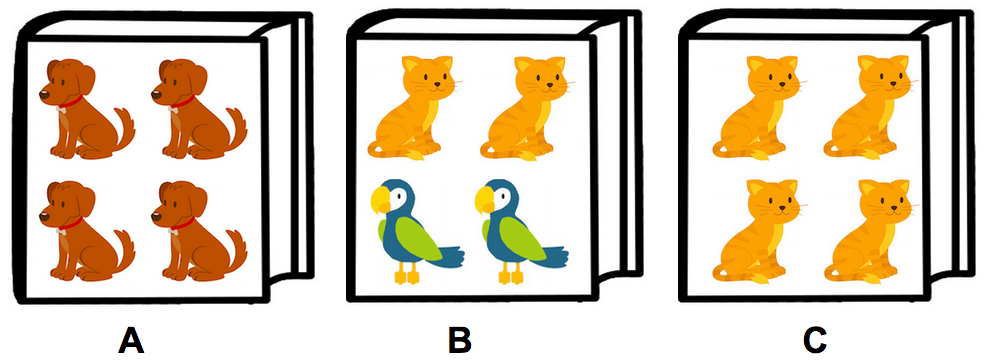
\includegraphics[height=1.25in]{figures/implicatures_demo_letters.png}
  \caption{\label{fig:demo} Example trial stimuli used in all experiments. Children received a clue from the experimenter about which book she had in mind and responded based solely on the clue; this was either an ad-hoc or a scalar description of a book with either an unambiguous or implicature target.}
 \end{center}
\end{figure}

 \begin{table*}
 \footnotesize
 \centering
     \begin{tabular}{C{1.5cm} C{2cm} C{1.5cm} C{1.5cm} C{4.5cm} C{1.5cm}}
                      \hline
       \null   Condition  & Trial type & \# trials, Expt. 1 & \# trials, Expts. 2 \& 3 & Statement: ``On the cover of my book, ...'' & Target   \\
       \hline
            Scalar & implicature & 4 & 6 &  ``...some of the pictures are cats'' & B	 \\
          & all  & 2 &  6 & ``...all of the pictures are cats'' & C		                 \\
           & none  & 2 & 6 & ``...none of the pictures are cats'' & A			\\
               & unambiguous `some' 	&  2 &  & ``...some of the pictures are birds'' & B					        \\
	\hline
	    Adhoc       & implicature & 4 &  & ``...there are cats'' & C 		\\
	     & distractor & 2 &  & ``...there are dogs'' & A	     \\
          & comparison & 2 &  & ``...there are birds'' & B 	   \\
       \hline
     \end{tabular}
     \caption{Study design for our scalar implicature task, using script examples for the stimulus set pictured in Figure \ref{fig:demo}. \label{tab:scripts} }
 \end{table*}

 \begin{figure}
 \begin{center}
  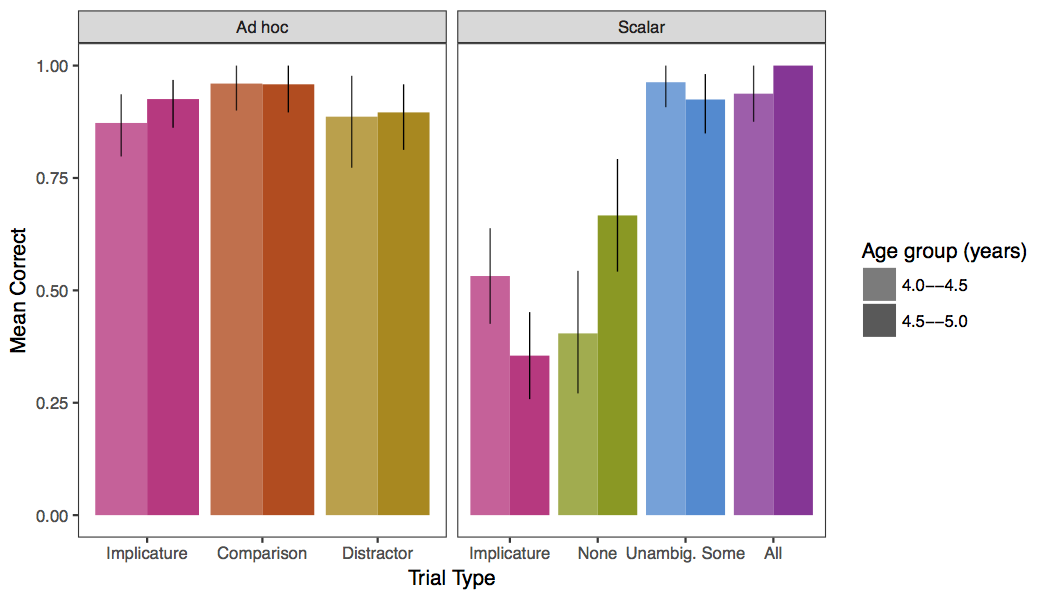
\includegraphics[width=4in]{figures/exp1_performance.png}
  \caption{\label{fig:exp1_perf} Proportion of correct responses by each age group across all trial types and split by implicature type for Experiment 1. Error bars show 95\% confidence intervals computed by non-parametric bootstrap.}
 \end{center}
\end{figure}

\begin{figure}
 \begin{center}
  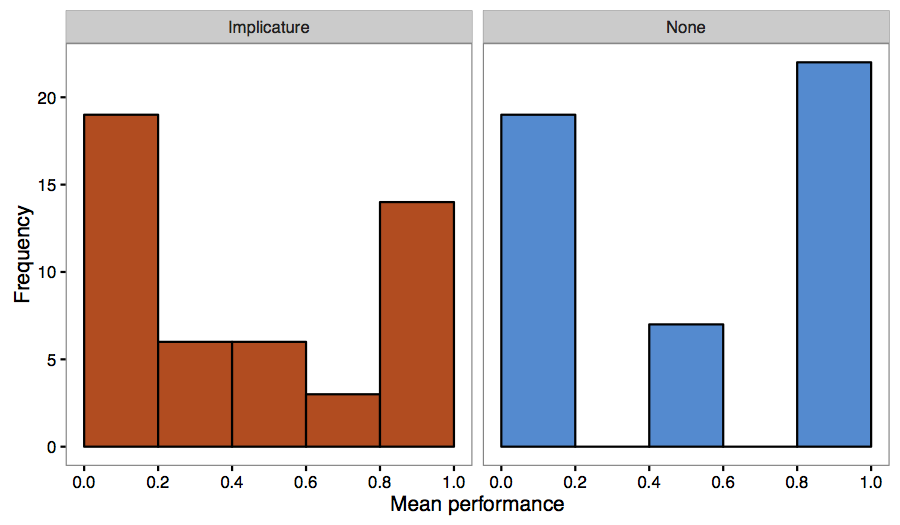
\includegraphics[width=4in]{figures/exp1_hist.png}
  \caption{\label{fig:imp_hist} Frequency of mean performance in Experiment 1, split by condition.}
 \end{center}
\end{figure}

\begin{table}
\centering
\begin{tabular}{ccccccc}
\hline
{\bf Age group} & {\bf N} & {\bf N Female} & {\bf N Male} & {\bf Mean} & {\bf Median} & {\bf SD} \\
\hline
3.0 -- 3.5-year-olds & 12 & 6 & 6 & 3.36 & 3.34 & 0.10\\
3.5 -- 4.0-year-olds & 13 & 5 & 8 & 3.67 & 3.67 & 0.12\\
4.0 -- 4.5-year-olds & 14 & 9 & 5 & 4.25 & 4.24 & 0.10\\
4.5 -- 5.0-year-olds & 12 & 3 & 9 & 4.67 & 4.62 & 0.15\\
\hline
\end{tabular}
\caption{\label{tab:exp_2_demo}Participant information for Experiment 2.}
\end{table}

\begin{figure}
 \begin{center}
  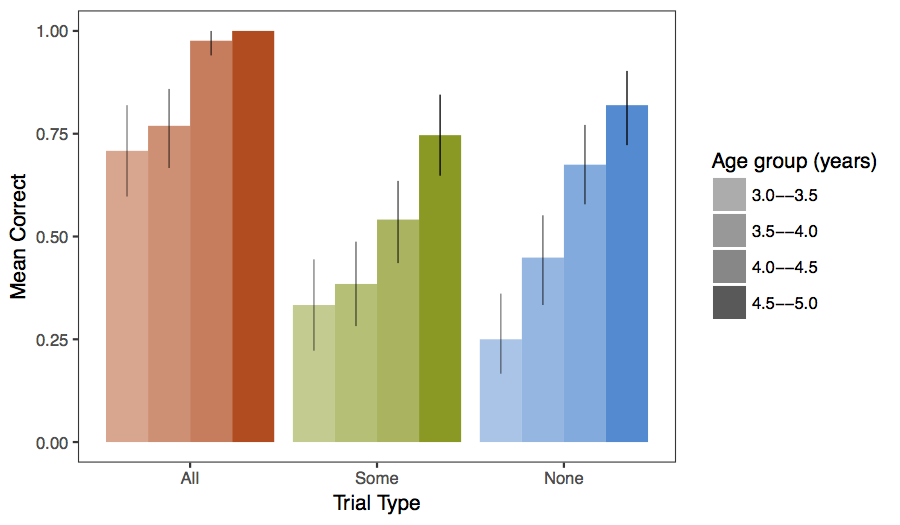
\includegraphics[width=4in]{figures/exp2_performance.png}
  \caption{\label{fig:exp2_perf} Proportion of correct responses by each age group across all scalar trial types for Experiment 2. Error bars show 95\% confidence intervals computed by non-parametric bootstrap.}
 \end{center}
\end{figure}

\begin{figure}
 \begin{center}
  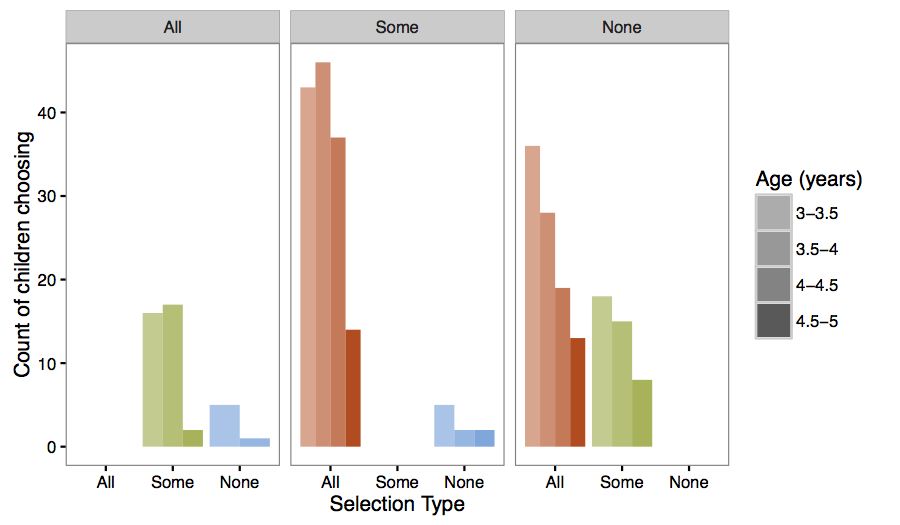
\includegraphics[width=4in]{figures/exp2_wrong.png}
  \caption{\label{fig:exp2_wrong} Scalar implicature error analysis for Experiment 2. Count of children choosing an alternative on incorrect trials, faceted by trial type (``all,'' ``some,'' and ``none'') and split by age group.}
 \end{center}
\end{figure}

\begin{table}
\centering
\begin{tabular}{ccccccc}
\hline
{\bf Age group} & {\bf N} & {\bf N Female} & {\bf N Male} & {\bf Mean} &  {\bf Median} & {\bf SD} \\
\hline
3.0 -- 3.5-year-olds & 18 & 12 & 6 & 3.23 & 3.24 & 0.13\\
3.5 -- 4.0-year-olds & 18 & 10 & 8 & 3.73 & 3.8 & 0.18\\
4.0 -- 4.5-year-olds & 18 & 7 & 11 & 4.15 & 4.11 & 0.11\\
4.5 -- 5.0-year-olds & 18 & 9 & 9 & 4.7 & 4.68 & 0.15\\
\hline
\end{tabular}
\caption{\label{tab:exp_3_demo} Participant information for Experiment 3.}
\end{table}

\begin{figure}
 \begin{center}
  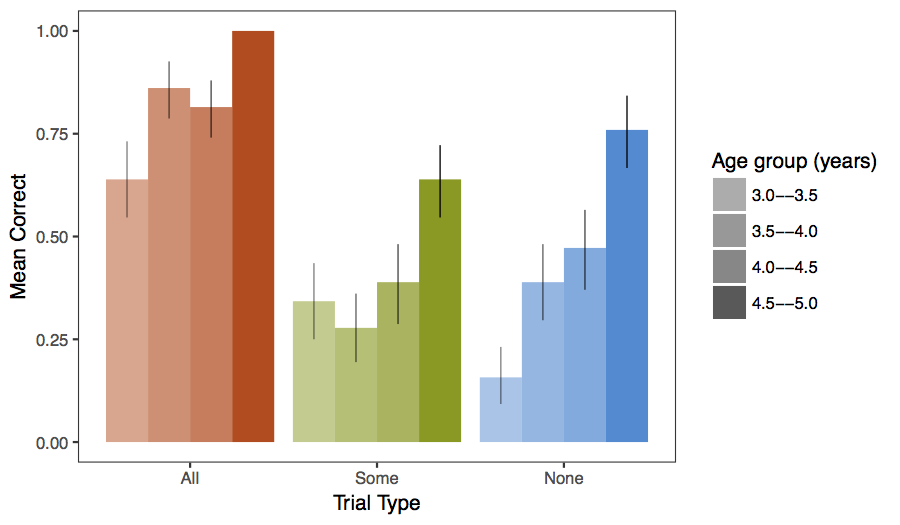
\includegraphics[width=4in]{figures/exp3_SIperformance.png}
  \caption{\label{fig:exp3_perf} Proportion of correct responses by each age group across all trial types for the scalar implicature task in Experiment 3. Error bars show 95\% confidence intervals computed by non-parametric bootstrap.}
 \end{center}
\end{figure}

\begin{figure}
 \begin{center}
  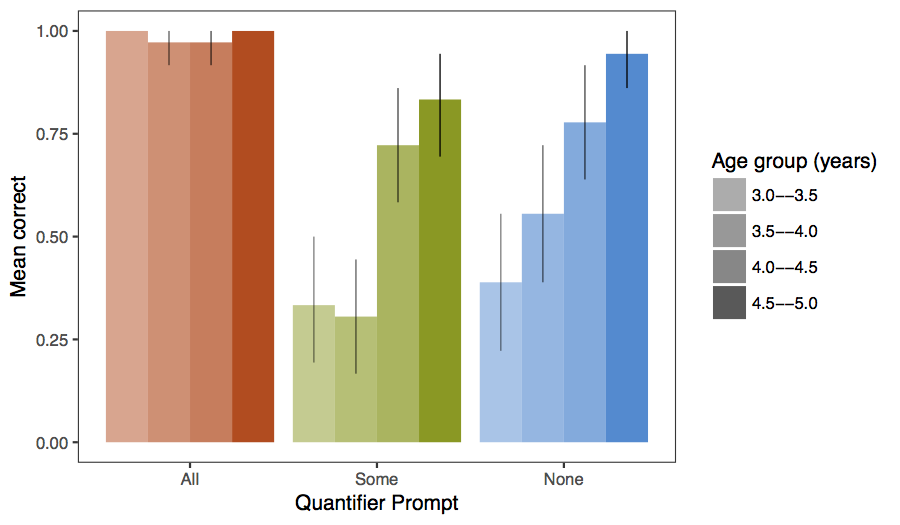
\includegraphics[width=4in]{figures/exp3_GQperf.png}
  \caption{\label{fig:exp3_GQright} Proportion of correct responses by each age group for the Give Quantifier task in Experiment 3, for quantifier prompts \textit{all, most, none} and \textit{some}. Error bars show 95\% confidence intervals computed by non-parametric bootstrap.}
 \end{center}
\end{figure}

\begin{figure}
 \begin{center}
  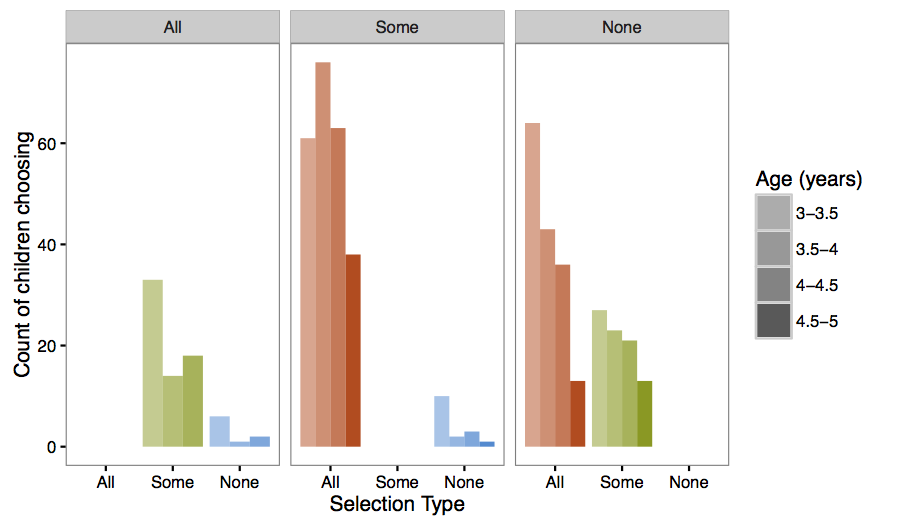
\includegraphics[width=4.5in]{figures/exp3_SIwrong.png}
  \caption{\label{fig:exp3_wrong} Scalar implicature error analysis for Experiment 3. Count of children choosing an alternative on incorrect trials, faceted by trial type (``all,'' ``some,'' and ``none'') and split by age group.}
 \end{center}
\end{figure}

\begin{figure}
 \begin{center}
  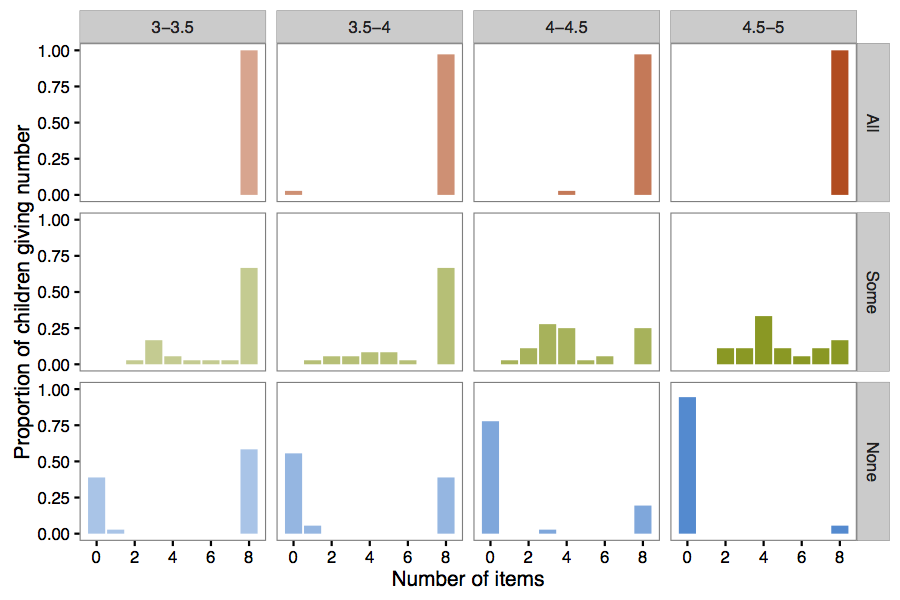
\includegraphics[width=4.5in]{figures/exp3_GQhist.png}
  \caption{\label{fig:GQ_spread} Give-Quantifier performance for Experiment 3. Proportion of children giving numbers of items faceted by age group and quantifier prompts (``all,'' ``none,'' and ``some'').}
 \end{center}
\end{figure}

\begin{table}
\centering
\begin{tabular}{ccccccc}
\hline
{\bf Age group} & {\bf N} & {\bf N Female} & {\bf N Male} & {\bf Mean} &  {\bf Median} & {\bf SD} \\
\hline
4.0 -- 4.5-year-olds & 18 & 14 & 4 & 4.23 & 4.22 & 0.14\\
4.5 -- 5.0-year-olds & 20 & 14 & 6 & 4.79 & 4.82 & 0.17\\
\hline
\end{tabular}
\caption{\label{tab:exp_4_demo} Participant information for Experiment 4.}
\end{table}


\begin{figure}
 \begin{center}
  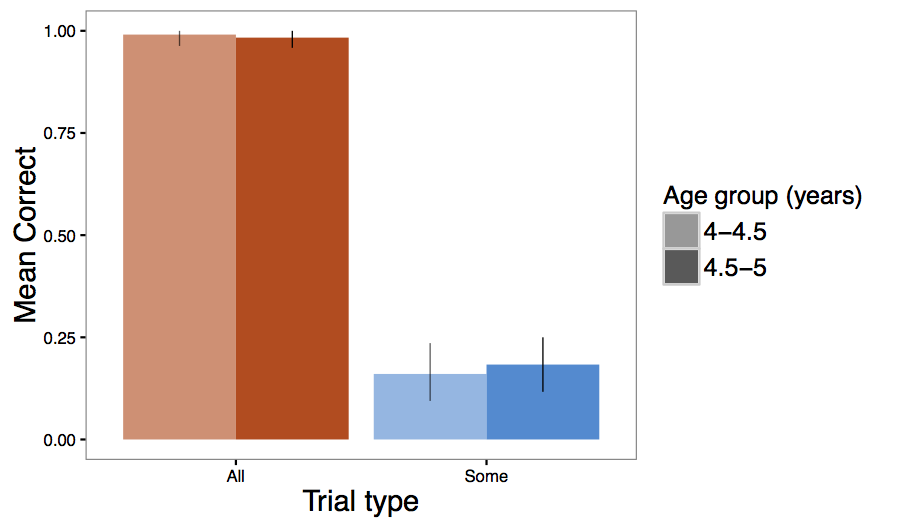
\includegraphics[width=4in]{figures/exp4_SIperf.png}
  \caption{\label{fig:exp4_si} Scalar implicature performance in Experiment 4. Plotting conventions are as above.}
 \end{center}
\end{figure}


%
%\bibliographystyle{apacite2}

\end{document}
